
% ----------EXAMPLES OF CITATIONS---------------- 
% I got a fact from \cite{fairfax_using_2018} and \cite{alakoski_distribution_2021}. I got another fact from this paper \parencite{bouwes_ecosystem_2016}. I also want to mention this paper. \footcite{bartak_spatial_2013}
% -----------------------------------------------

Economic production faces environmental conditions that threaten efficiency. Technology and industrial partially neutralize the threat (for instance, irrigation enabling productive agriculture in arid regions), but economically desirable solutions may harm social welfare. One salient example is the conflict between wildlife and agriculture. The success of farming operations has often hinged on the ability of the producer or its government to cull livestock predators and crop grazers, repel potential vectors of disease, and eliminate crop-eating pests with mass insecticide use. Such measures, however, may produce both ecologically and socially undesirable outcomes. Case studies abound. In the past two decades, the US Department of Agriculture's Wildlife Services has killed 56 million wild animals, including some otherwise protected by the Endangered Species Act, to protect agricultural assets, largely livestock (VOX CITE). Pesticides used to protect crop yields negatively impact human and animal health \citep{larsen_agricultural_2017}, leading in part to the formation of the modern American environmental movement \citep{woodwell_broken_1984}. The Chinese ``Four Pests Campaign'' encouraged the mass killing of sparrows, believed to feed on grain reservoirs, and inadvertently eliminated sparrows' valuable pest-control services, playing a role in the subsequent mass famine (CITE). 

Balancing economic production and ecosystem protection is complicated by climate change, habitat destruction, and biodiversity loss \citep{cardinale_biodiversity_2012}. Indeed, misunderstanding the role keystone species play in supporting their ecosystems can distort wildlife management policy; recent evidence has challenged long-held beliefs about so-called ``nuisance'' species (e.g., \cite{raynor_wolves_2021}). There remains, however, scant empirical evidence on the economic impacts of targeted wildlife on agricultural functioning.

The beaver (\textit{Castor canadensis} in North America\footnote{Kuhl, 1820} and \textit{Castor fiber} in Europe and Western Asia\footnote{Linnaeus, 1758}) occupies the dual roles of agricultural menace and crucial ecosystem engineer. Since the expansion of agricultural in Europe and America, farm operators have often resorted to beaver killing to avoid the flooding, crop grazing, and timber felling associated with beaver habitation. After being hunted to near-extinction until the 19th Century, the beaver has been reintroduced in many parts of North America and Europe. In recent years, a plethora of positive externalities produced by beavers has been well-documented, from wetland preservation \citep{hood_beaver_2008}, temperature regulation (\cite{dittbrenner_relocated_2022}), and carbon storage (\cite{wohl_landscape-scale_2013}, \cite{johnston_beaver_2014}) to wildfire resistance \citep{fairfax_smokey_2020} and the flourishing of species richness \citep{wright_ecosystem_2002}.

A recent unplanned, unsanctioned reemergence of beavers in Scotland, where they had not appeared in several centuries, illustrates this conflict. Consistent with historical examples of farmer-led opposition to beaver habitation, agricultural groups have pushed back against the incursion into the agriculturally valuable region around the River Tay (hereafter, ``Tayside''), with the president of the National Farmers Union, Scotland (NFUS) warning that beavers pose a greater threat than Brexit to his constituents \citep{castle_beavers_2021}. In nearby Southern England, which has seen several controlled releases, residents have posted public banners vowing to oppose beaver invasion (cite). Despite this staunch opposition, Scotland granted beavers protected status in 2019, restricting farmers' latitude to kill occupying beavers at will.

The case of the Scottish beaver can inform wildlife management policy. Exogenous to agricultural policy, climate change,\footnote{Not all beaver expansion has been uncorrelated with the identification-confounding effects of climate change. In recent decades, the warming Arctic tundra has proved fertile habitat for beavers \citep{tape_expanding_2022}, which are further altering the environment via their colonies' methane production \citep{clark_beaver_2023}} or wildlife management regime shifts, the illegal arrival and rapid spread of the beaver in Scotland  allows one to estimate the causal impact on agricultural land use.

I employ a set of periodic comprehensive regional surveys, undertaken between 2012 and 2020, to identify beaver presence and movement. To test whether beaver presence affects agricultural outcomes, I match high-resolution land use data to beaver arrival. Because multiple channels exist by which beavers may harm agricultural operations, I provide suggestive evidence for the most commonly cited mechanism: flooding. Using a dense network of hydrometry monitoring stations across Scotland, I changes in river level and flow in response to beaver presence.

I find mixed evidence for beaver impacts. In my preferred specification, beaver arrival is associated with a 1.7 p.p. \textit{increase} in the share of landscape grid cells devoted to agricultural land use, a 13.6\% change relative to the average agricultural land share. River level averages reduce modestly and insignificantly, while level maxima (i.e., the highest level measured in a given month) rises slightly, though not significantly. In preliminary analysis, it remains unclear whether the increased share of land devoted to agricultural use ``caused" by beaver entry reflects true changes in cropping, or rather the greening effect of beaver colonization. Further study, using satellite data to measure water-saturation and flooding events directly at a finer scale, as well as agricultural census data on farm productivity and income, will help clarify the causal relationship.

This paper makes three main contributions. First, it builds on a small existing literature quantifying the economic impacts of wildlife on economic production.

Second, it contributes to the literature, largely in ecology, wildlife biology, and environmental policy, on the successful management of reintroduced species, with particular attention to avoiding human-wildlife conflict

Third, it adds to existing literature in economics on agricultural damage response functions, particularly in response to natural disasters and adverse environmental conditions.

The paper is structured as follows Section \ref{sec:background} briefly describes beaver ecology, agricultural production in Scotland, and the reemergence, in the 2000s, of beavers in Scotland. Section \ref{sec:data} reviews the data. Section \ref{sec:methods} describes my empirical approach, including data construction and regression specifications. Section \ref{sec:results} presents results on reduced-form beaver impacts on agriculture, as well as suggestive evidence on mechanisms. Section \ref{sec:discussion} discusses implications for policy. \ref{sec:conclusion} concludes and points toward future research. 

\begin{figure}
    \centering
    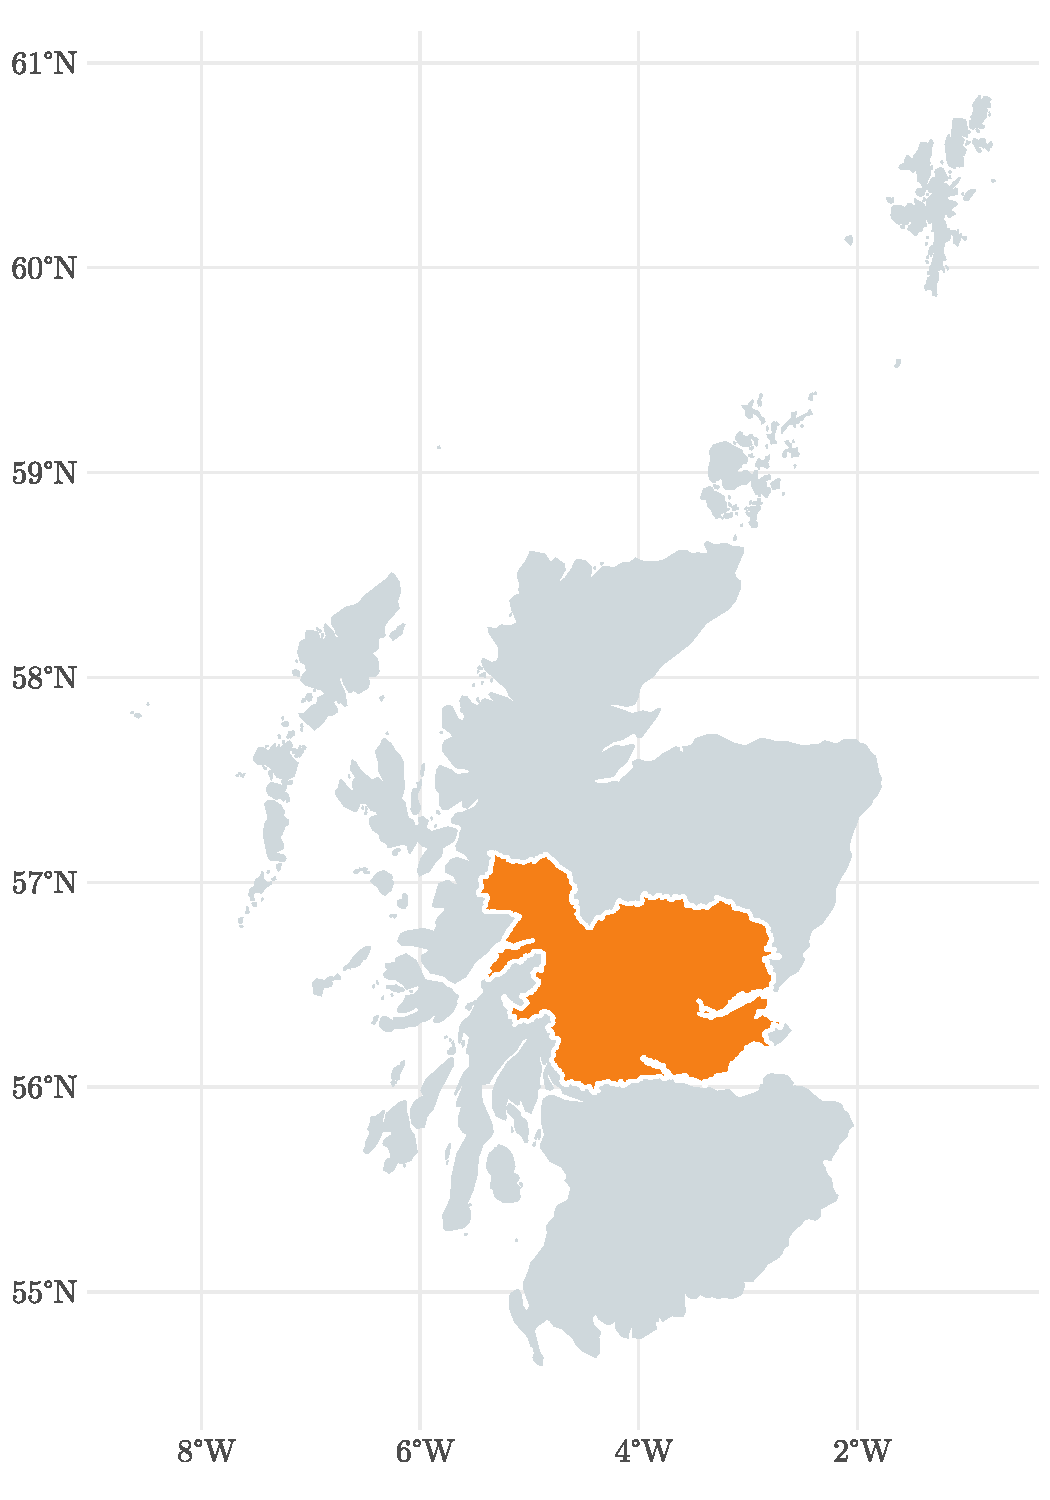
\includegraphics[width=0.5\linewidth]{output/figures/study_area.pdf}
    \caption{Study region (orange) within Scotland. Agricultural parish boundaries are drawn in gray.}
    \label{fig:enter-label}
\end{figure}

\begin{figure}
    %\centering
    \begin{subfigure}{0.39\linewidth}
        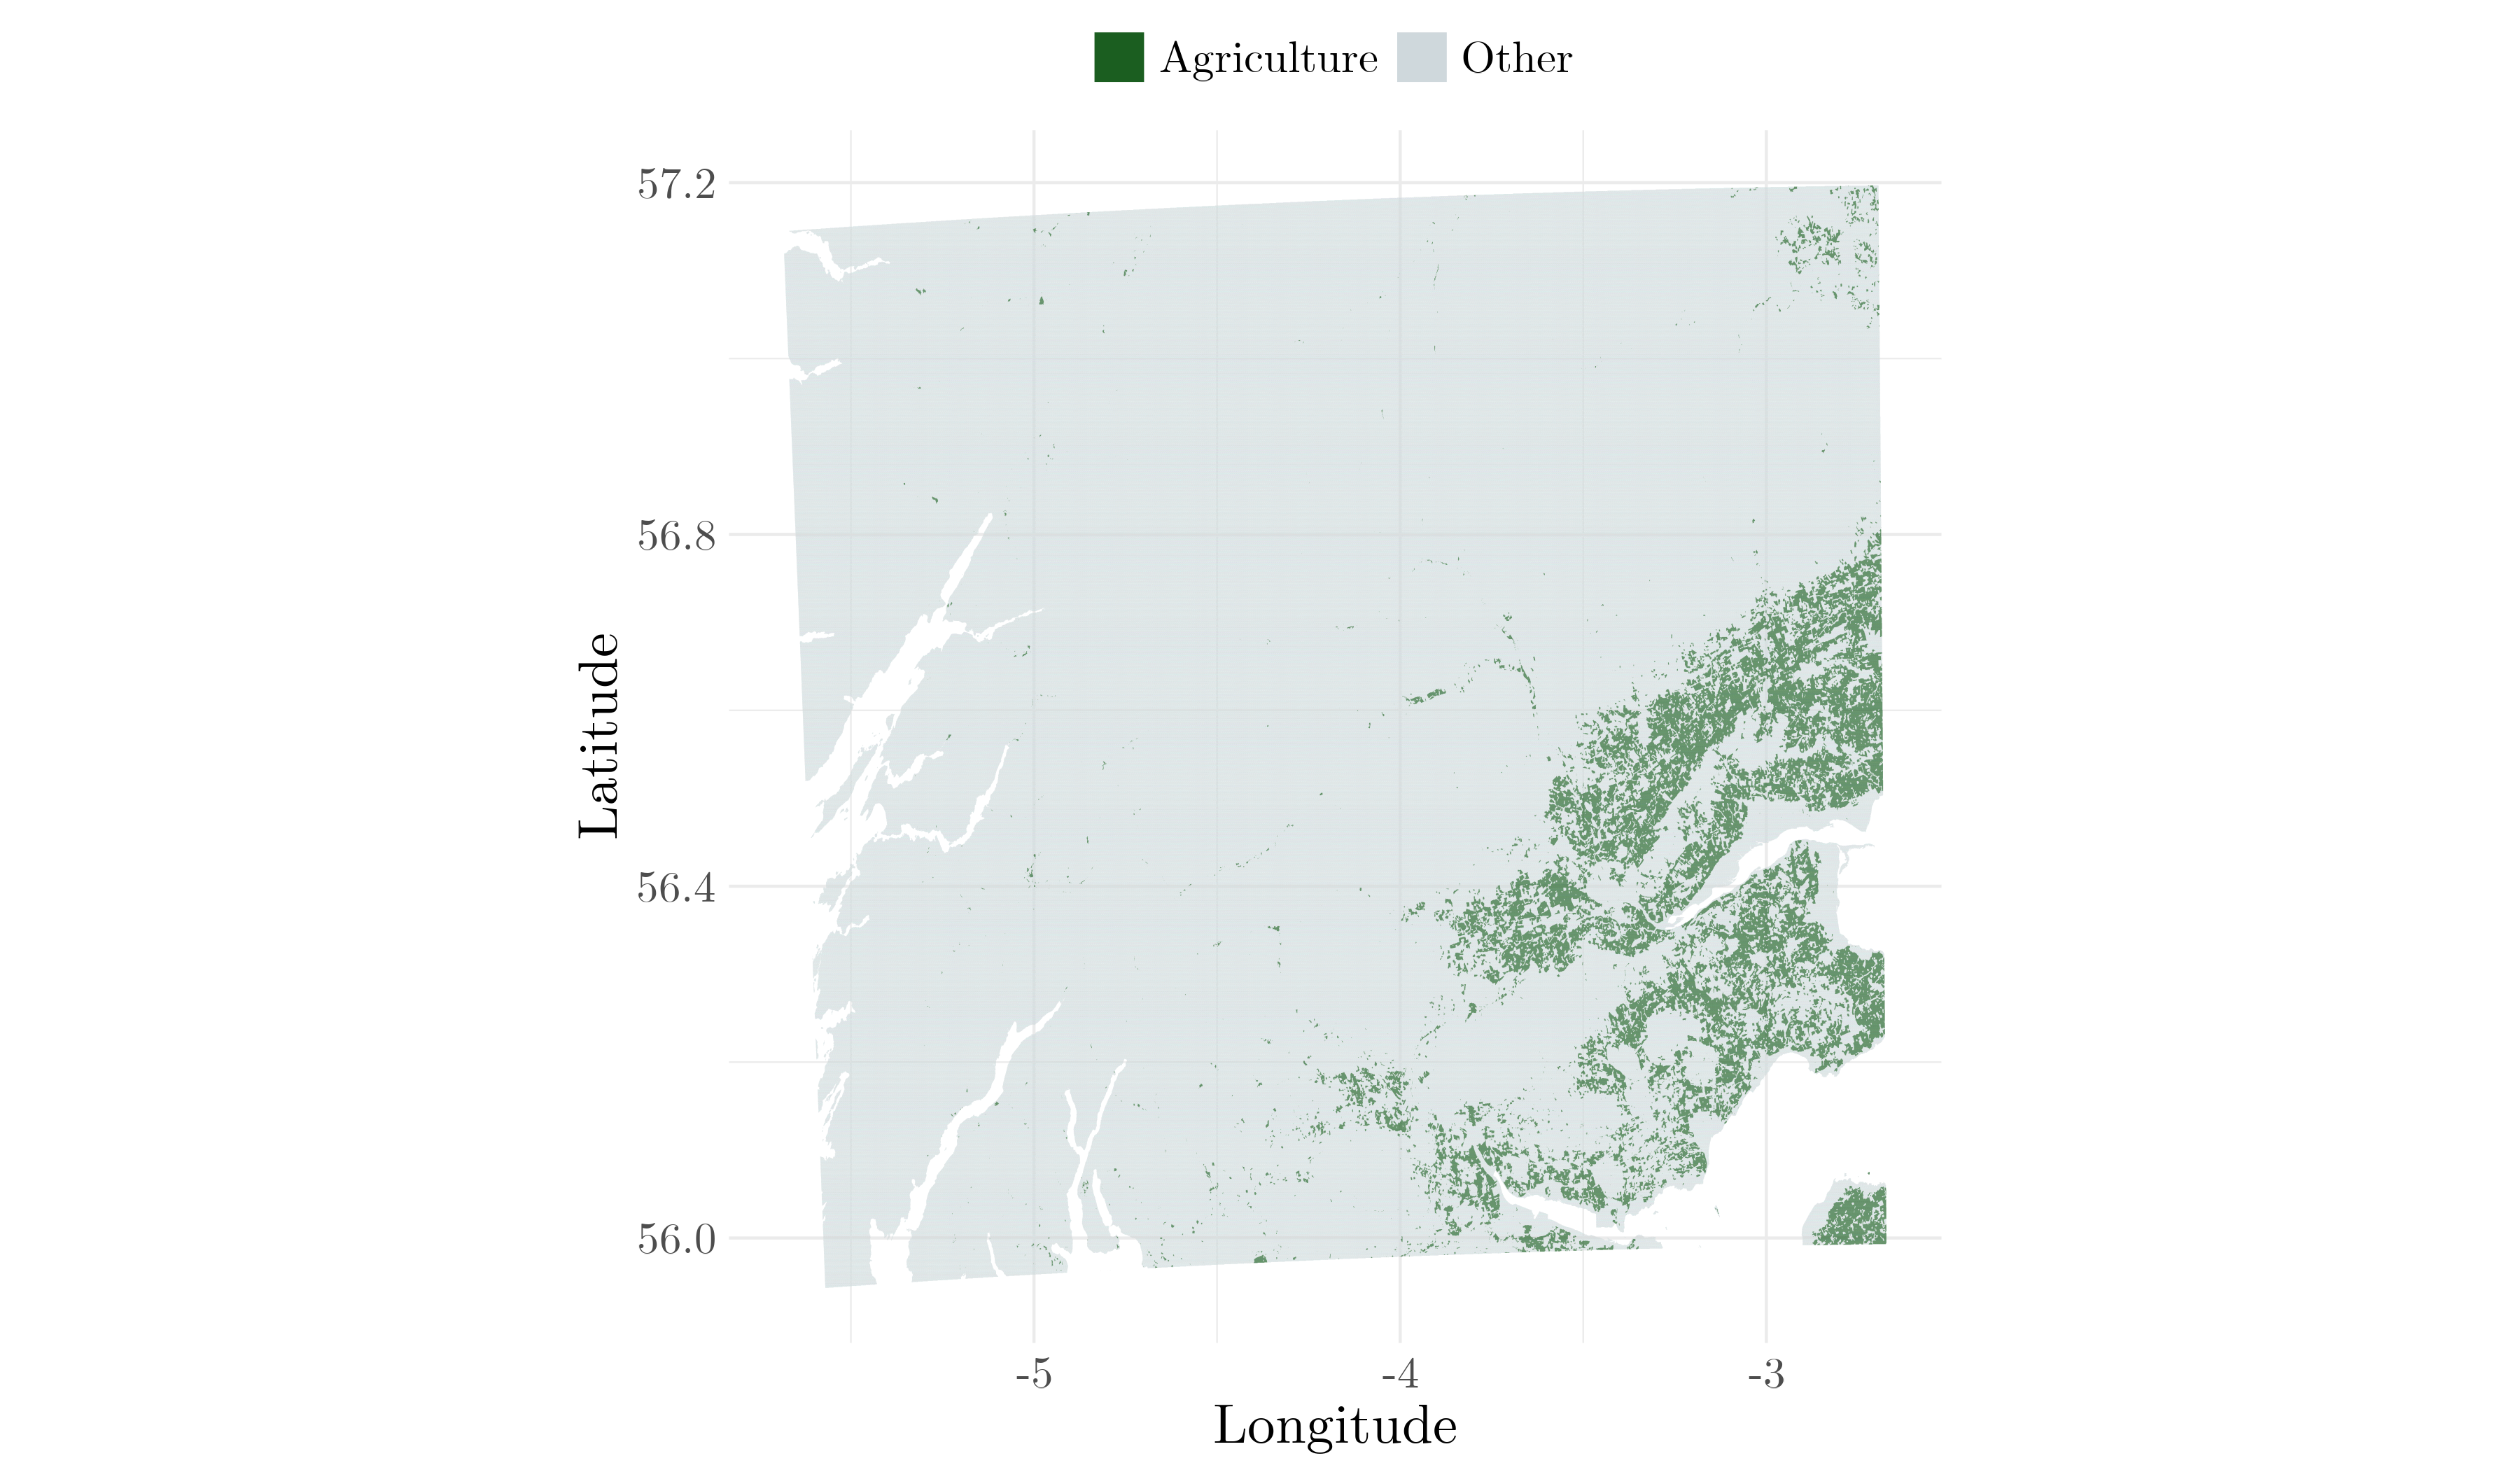
\includegraphics[width=\linewidth]{output/figures/lcm_in_study_area.png}
        \caption{25m raster cells classified as agricultural (``arable'' in UKCEH nomenclature)}
        \label{fig:ukceh-lcm-raw}    
    \end{subfigure}
    \begin{subfigure}{0.6\linewidth}
        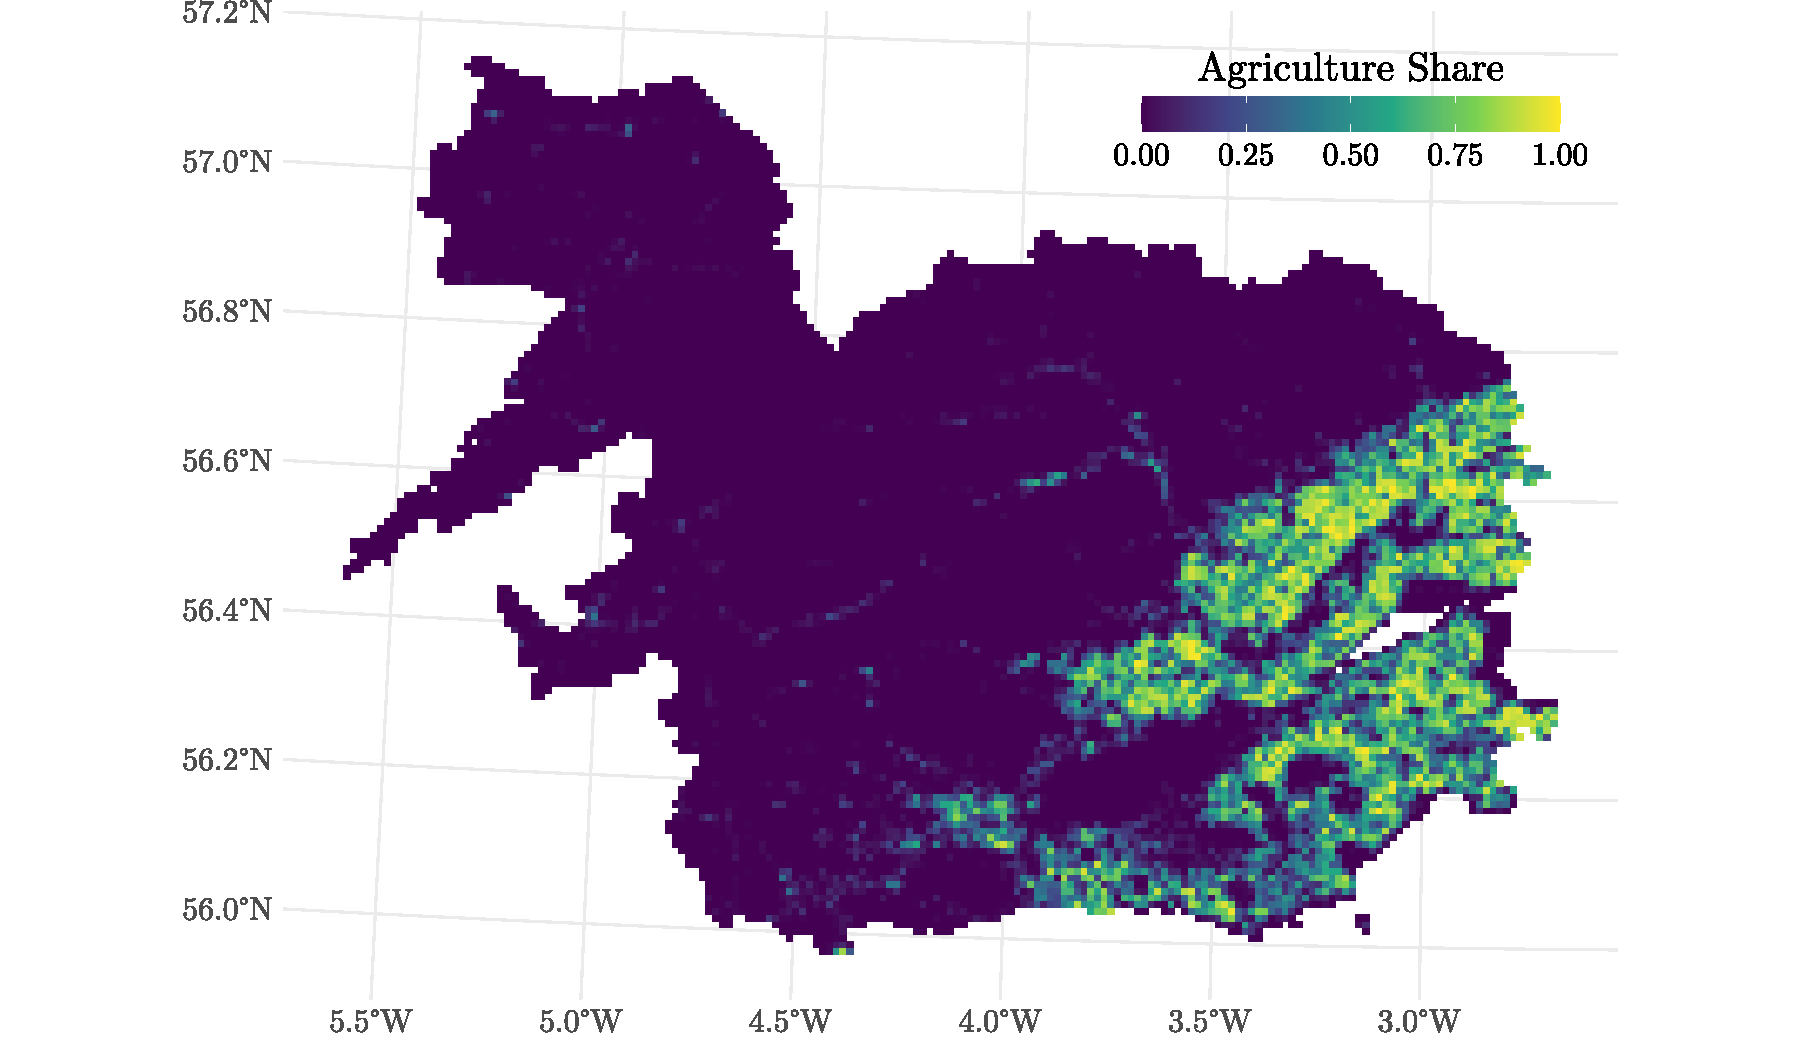
\includegraphics[width=\linewidth]{output/figures/lcm_agg_river_grid.pdf}
        \caption{Agricultural raster layer aggregated to 1km$^2$ landscape grid cells in study region.}    
        \label{fig:ukceh-lcm-agg}
    \end{subfigure}
    \caption{Agricultural land use in 2022. Data source: UK Center for Ecology \& Hydrology. See main text for details.}
\end{figure}

\begin{figure}
    \centering
    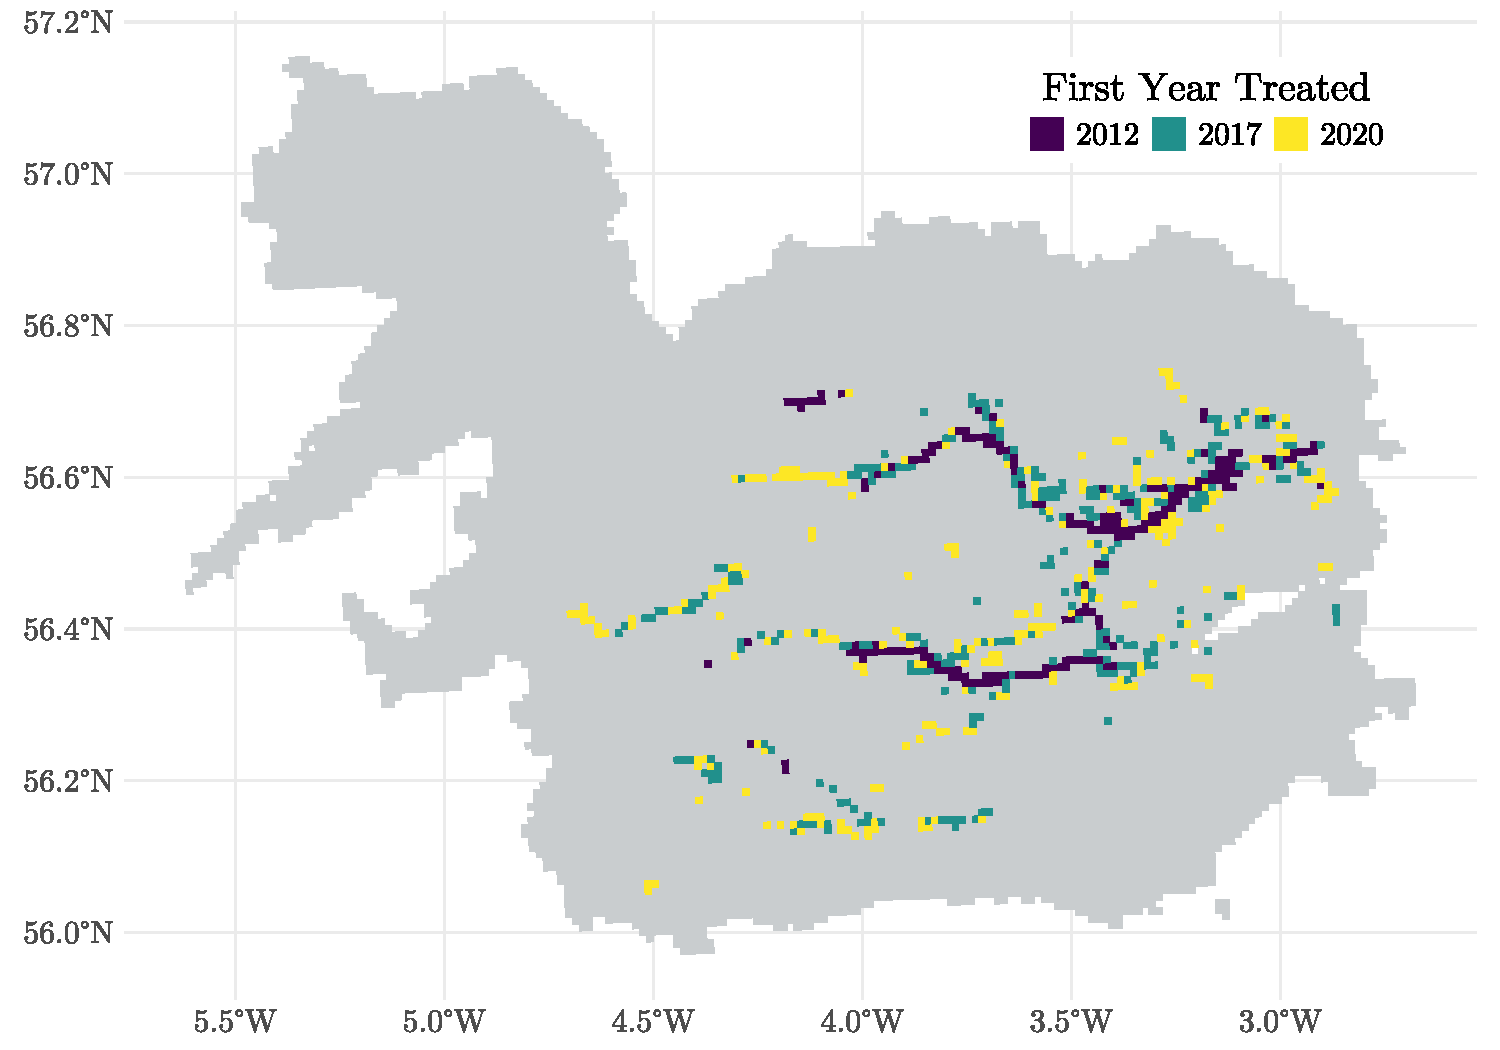
\includegraphics[width=0.7\linewidth]{output/figures/beaver_first_year_treated.pdf}
    \caption{Beaver detection by survey year in study region. Observation units are 1km$^2$ landscape grid cells. Data source: See main text for details.}
    \label{fig:enter-label}
\end{figure}


% \begin{itemize}
%     \item In the face of climate change, habitat destruction, and biodiversity loss, there is a lot of focus on wildlife reintroductions.
%     \item In many cases, reintroduced wildlife will interact with the human environment, producing a range of positive and negative externalities (spreading disease, predators that eat livestock, highway collisions, ecology-disrupting brumbies, etc.). 
%     \begin{itemize}
%         \item These conflicts with human environments is due, in part, to the history of human development going hand in hand with the destruction of wild habitats (e.g., draining swamps to establish agriculture). 
%     \end{itemize}
%     \item One salient example are the ongoing conflicts over the coexistence of human agriculture and the beaver, an ecosystem engineer which alters the course of rivers, establishes wetlands, fells timber, and grazes on vegetation. While the benefits of beaver presence have been well-documented, reliable cost estimates are rare. Farmers are a frequent opponent to beaver presence (cite examples from the beaver conflict literature). In Scotland, farmers have expressed dismay over a recent reemergence of beavers (here, give context for Kennedy Brexit quote).  
%     \item The recent unplanned, unauthorized establishment of a now-massive beaver population in the agriculturally valuable Scottish region around the River Tay (hereafter, ``Tayside'') presents a valuable natural experiment to estimate the general impact of beaver habitation on agricultural viability. Exogenous to ag policy, climate change (compare to Arctic expansion \citep{tape_expanding_2022}), or wildlife management regime.
%     \item To my knowledge, only one study has assessed the agriculture impacts of the Tayside beavers \citep{hamilton_tayside_2015}. Detail how this paper expands on and improves Scott's estimation procedure.
%     \item Using data on beaver expansion, agricultural activity, and river levels, I estimate the impact of the Tayside beavers on a range of farm outcomes.
%     \item I find \textcolor{red}{X} effect.
%     \begin{itemize}
%         \item Compare my estimates to \citep{hamilton_tayside_2015} and others.
%     \end{itemize}
%     \item I contribute to the literature on:
%     \begin{itemize}
%         \item Beaver costs and benefits
%         \item More broadly, wildlife reintroductions and cohabitation. 
%         \begin{itemize}
%             \item (cite a few examples of small-scale estimates, like \citep{hamilton_tayside_2015}. Maybe mention this\footnote{Mention \href{https://www.exeter.ac.uk/media/universityofexeter/research/microsites/creww/riverottertrial/appendix1/Beavers_and_Agriculture.pdf}{this} as an example and note that it was in the context of a minuscule and more controlled beaver population. In addition, the estimates are only at a few sites})
%         \end{itemize}
%         \item Agricultural damage response functions
%     \end{itemize}
    
% \end{itemize}